\chapter{Methodology}
\label{chapterlabel4}

This section describes the procedures used to collect data and conduct the analysis that was employed to answer the research question in this study. We begin by describing the process of selecting case studies. We then detail our process of collecting and cleaning relevant historical OSM data. We detail the empirical approach used to analyze and visualize this data to gain a greater understanding of processes of humanitarian mapping and subsequent data maintenance efforts. Throughout this process, our approach to analysis was largely exploratory and iterative. We tested a variety of approaches for aggregating, subsetting, querying, and visualizing the many variables included in our datasets. We considered each case study (mapping activation) to be our \textit{unit of analysis}, within which our \textit{unit of observation} was a unique OSM entity that was created during a given mapping activation. All data processing and analysis was done using the Java and R programming languages.

\section{Case study selection}

The scope of this work is limited to four humanitarian mapping case studies and one reference case study. We selected humanitarian case studies that consisted of mapping efforts in response to a humanitarian need, were constrained to subnational geographic areas, drove a sufficient volume of mapping activity on OSM (as defined by volume of unique contributors and volume of edits over time), and were sufficiently documented on pages such as the OSM Wiki\footnote{\url{https://wiki.openstreetmap.org/wiki/Main_Page}}, HOT Projects page\footnote{\url{https://www.hotosm.org/projects/}}, or HOT Tasking Manager\footnote{\url{https://tasks.hotosm.org/}}. We have also selected case studies that capture practices of humanitarian mapping at various stages in the history of the humantiarian OSM community. However, we have not selected any cases that have occurred within the last five years, to allow for the study of maintenance practices in the years following a mapping activation.  

Following from the above criteria, we focus on humanitarian mapping activities in 1) Port au Prince, Haiti, following the 2010 earthquake, 2) Tacloban, Philippines, following the 2015 typhoon, 3) Bangui, Central African Republic, following 2013 rebellions, and 4) Kathmandu, Nepal, following the 2015 earthquake. In addition to these four humanitarian case studies, we have also selected a 'reference' case study as a contrasting example of mapping activities in a region with a highly active and matured OSM community. Following \textcite{anderson_crowd_2018}, we select Heidelberg, Germany as our reference case.

\section{Processing historical OSM data}
\label{sec:history}

Unprocessed OSM historical data extracts for each case study area were downloaded from Geofabrik.\footnote{\url{http://download.geofabrik.de/}} This 'raw' data was then processed using the OSHDB framework \parencite{raifer_oshdb_2019}. OSHDB was selected due to the speed and flexibility that it provides in processing and filtering historical OSM data. Despite these advantages offered by the OSHDB framework, the complexity of OSM history data means that the extraction of relevant variables constituted a significant portion of this methodology. 

%%%%%%%%%%%%%%%%%%%%%%%%%% Over time image 
\begin{figure} % opens the figure environment. the '[H]' forces the image to be Here
    \centering % puts the image in the horizontal centre of the page
    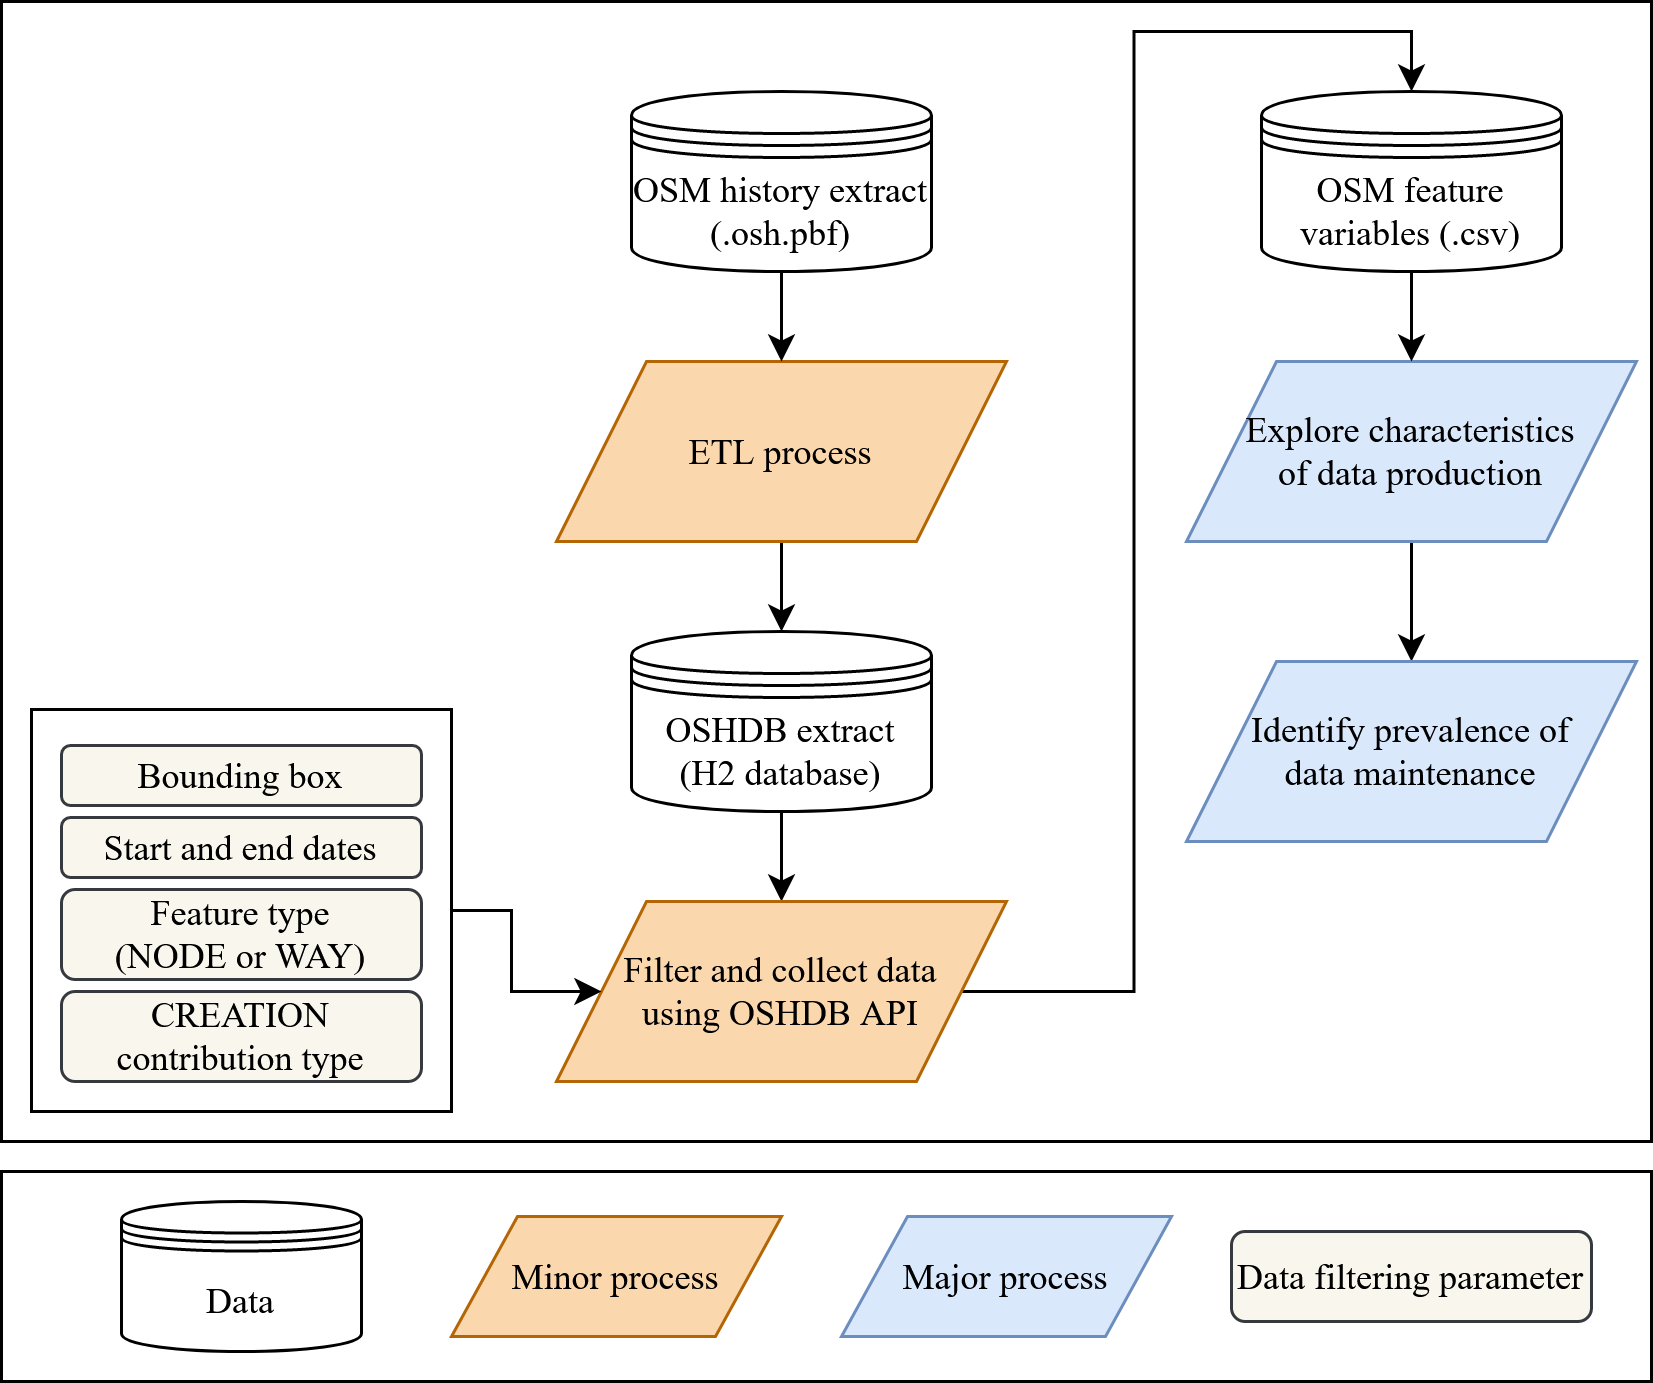
\includegraphics[width = \textwidth]{Images/Datapipeline.png} %this tells latex what graphics to include. 
    \caption{Summary of data processing pipeline} % this prints the caption below the figure
    \label{fig:pipe} % this internally labels the figure for future referencing.
\end{figure}
%%%%%%%%%%%%%%%%%%%%%%%%%% 

To begin, each OSM history extract, in \textit{.osh.pbf} format, was converted to a local OSHDB instance, following the Extract, Transform, Load (ETL) process described in the OSHDB documentation.\footnote{\url{https://github.com/GIScience/oshdb/tree/master/oshdb-tool/etl}} This process loads the data from each extract into separate local H2 databases that are hosted locally. Each OSM entity is transformed into an OSH entity, a data format designed for use within the OSHDB framework. OSH entities allow for more efficient storage of OSM data as they group together different versions of the same entity \parencite{raifer_oshdb_2019}. We note that some of the historical extracts were too large to be processed locally in this manner and so technical assistance in generating some extracts was provided by a researcher from the Heidelberg Institute for Geoinformatik Technology (HeiGIT) team. 

The OSHDB API \parencite{raifer_oshdb_2019} was then used to filter and process the historical data to obtain variables of interest.  Implemented in the Java programming language, this API allows for data filtering and aggregation based on the \textit{MapReduce} programming framework \parencite{raifer_oshdb_2019}. This framework is designed for use with large datasets and contains a \textit{map} function whereby data is filtered and sorted, followed by a \textit{reduce} function whereby data is summarized and returned as aggregated values \parencite{dean_mapreduce_2008}.

We collected data for each case study using the spatial and temporal extents specified in Table \ref{tab:cases}. Bounding boxes correspond to the smallest square area encompassing the city of interest (here with coordinates rounded to two decimal places for greater legibility). The start and end date for each of the humanitarian activations was collected from the associated HOT project page.\footnote{\url{https://www.hotosm.org/projects/}} The start and end dates for the Heidelberg reference case were selected to cover a year-long period that was relatively early in the development of the map for this area, to be better compared against the humanitarian cases. 

%%%%%%%%%%%%%%%%%%%%%%%%%% TABLE 
\begin{table}
\centering
\caption{Summary the spatial and temporal extent used to filter data for each case study}
\label{tab:cases}
\begin{tabular}{llll}
\toprule
Name                     & Start      & End        & Bounding box                 \\
\midrule
Heidelberg               & 2008-12-31 & 2009-12-31 & 8.57, 49.35, 8.79, 49.46     \\
Port au Prince         & 2010-01-12 & 2011-10-31 & -72.57, 18.34, -72.16, 18.63 \\
Bangui & 2013-03-23 & 2015-12-31 & 18.49, 4.32, 18.59, 4.49     \\
Tacloban           & 2013-11-10 & 2014-01-31 & 124.89, 11.18, 125.08, 11.34 \\
Kathmandu         & 2015-04-25 & 2015-12-31 & 85.27, 27.67, 85.38, 27.75  \\
\bottomrule
\end{tabular}
\end{table}
%%%%%%%%%%%%%%%%%%%%%%%%%%

For each of the case studies, we focused solely on the new data that was produced and disregarded any modifications to existing data. We also focused only on nodes and ways, given that these are the most common OSM entities (disregarding relations), particularly in humanitarian mapping efforts. Thus using the OSHDB's \textit{stream()} functionality, we collected numerous variables from all OSM entities that were created during this time, and all subsequent versions of these entities that were created in the time following the mapping activations. For example, we collected the details about the OSM entity, \textit{Node X}, that was created during the mapping efforts in \textit{Case Study Y}. Here, \textit{Node X} would have a version \#1. By grouping together all versions of a given OSM entity within a parent OSH entity, the OSHDB data model also allowed us to collect information from all subsequent versions of \textit{Node X}. These subsequent versions reflect modifications that were made to \textit{Node X} after it was initially created, such as modifications to its geometry or tags. The variables collected for each OSM entity are summarized in Table \ref{tab:vars}. 

The information captured by these variables is diverse, encompassing numerical, spatial, temporal, and attributional information. We also note that, while most variables are highly structured, the information contained within the \textit{Tags} variable requires significant cleaning to be useful. Across all case studies, we have collected data from 308,147 OSM entities. Due to the presence of multiple versions for some entities, as described above, we note that not all of these entities were created during times of each mapping activation, as detailed in Table \ref{tab:cases}.

%%%%%%%%%%%%%%%%%%%%%%%%%% TABLE 
\begin{table}
\centering
\caption{Summary of variables collected from OSM entities}
\label{tab:vars}
\begin{tabular}{lll}
\toprule
Variable       & Description                                                                                    & Data type   \\
\midrule
ID             & Unique identifier for OSM/OSH entity                                                           & Numeric     \\
User ID        & The user ID of the OSM contributor                                                             & Numeric     \\
Bounding box   & Bounding box for the OSH entity                                                                & Coordinates \\
Type           & Node or way                                                                                    & Text        \\
Version number & Version number for the OSM entity                                                              & Numeric     \\
Timestamp      & Time of entity creation                                                                        & Date/time   \\
Tags           & \begin{tabular}[c]{@{}l@{}}Tags and keys associated with the \\ OSM entity\end{tabular}        & Text        \\
Visibility     & \begin{tabular}[c]{@{}l@{}}Indicating whether or not the \\ node has been deleted\end{tabular} & Boolean  \\
\bottomrule
\end{tabular}
\end{table}
%%%%%%%%%%%%%%%%%%%%%%%%%%

\section{Exploring the characteristics of data production}
\label{sec-production}

This historical OSM data was then analyzed to understand the basic characteristics of data production for each mapping activation. We performed numerous data processing steps to understand how the data was produced over time, where the data was produced over space, what sources contributed to data production, and what types of geographic entities were produced. We also calculated numerous summary statistics for each case study to allow for quantitative comparison.

To understand the dynamics of data production over the duration of each mapping activation, we aggregated all entities by the day that they were produced. We calculated the total number of entities produced and the unique number of contributors each day. We then calculated the relationship between these two variables, by day, using the Pearson correlation coefficient. 

We investigated the patterns of data production over space by visualizing the density of new entities created within each study area. Following \textcite{grochenig_estimating_2014}, we used tessellation of hexagons to bin all data points within uniform polygons, allowing for easier comparison across case studies. The authors cite \textcite{hagenauer_mining_2012} in claiming that the hexagon shape is also well-suited to visualizing phenomena in urban areas. We calculated the centroid from each entity's bounding box to create this point-based density visualization. 

We parsed the tags associated with each entity to understand the types of features that were mapped and their associated sources. While tagging conventions within the OSM community result in many standardized tags used across entities, we conducted some basic text preprocessing to ensure that all text was normalized as much as possible, allowing for more accurate aggregation. We converted all characters to lowercase and removed non alpha-numeric characters. For each case study, we calculated the most frequently occurring tag keys (and not the associated values) to provide an indication of the types of features that were mapped. We also analyzed the values that are associated with the 'source' tag key across entities as in \textcite{ahmouda_analyzing_2018}. While no longer a common tagging practice, the 'source' tag key has frequently been used within the OSM community as a way to indicate the information source behind a given contribution \parencite{noauthor_keysource_nodate}. For example, entities that were added to OSM by tracing Bing satellite imagery might be accompanied by the \texttt{source=Bing} key-value pair. We calculated the most frequently occurring source values for each case study to provide an indication of the common information sources (particularly to indicate remote vs local sources). 

In addition to the above analyses, we calculated various metrics to provide a basis for empirical comparison between case studies. These metrics are summarized in Table \ref{tab:metrics}. We follow \textcite{anderson_crowd_2018} and \textcite{haklay_how_2010} in calculating the contributor density for each case study, as an indication of the quality of contributions. We additionally calculate the density of contributions (entities created). Given that our case studies encompass areas of different sizes, these density calculations normalize values, allowing for better comparison across cases. We also follow \textcite{dittus_mass_2017} in calculating the 'burstiness' of each case study and classifying each case study as an event or mission. The burstiness measure provides insight into the dynamics of data production and is particularly relevant in the context of humanitarian mapping, as data is often produced very quickly over time in response to a crisis \parencite{dittus_mass_2017}. 

%%%%%%%%%%%%%%%%%%%%%%%%%% TABLE 
\begin{table}
\centering
\caption{Metrics calculated to compare mapping activity across case studies}
\label{tab:metrics}
\begin{tabular}{lll}
\toprule
Metric                      & Unit                               & Formula                                                                                                                  \\
\midrule
Duration                    & \(days\)                               & End date - start date                                                                                                    \\
Area                        & \(km^2\)             & Bounding box length * width                                                                                              \\
Total entities created      & \(entities\)                           & NA                                                                                                                       \\
Density of entities created & \(entities/km^2\)      & Total entities/area                                                                                                      \\
Total unique contributors   & \(contributors\)                       & NA                                                                                                                       \\
Density of contributors     & \(contributors/km^2\) & Total contributors/area                                                                                                  \\
Burstiness                  & \(days\)                               & \begin{tabular}[c]{@{}l@{}}Number of days until 50\% of all \\ contributions were made\end{tabular}                      \\
Activation style            & \textit{EVENT} or \textit{MISSION}                   & \begin{tabular}[c]{@{}l@{}}Event if burstiness \textless 60, or \\ Mission if burstiness \textgreater{}= 60\end{tabular} \\
\bottomrule
\end{tabular}
\end{table}
%%%%%%%%%%%%%%%%%%%%%%%%%%

Through the analysis described in this section, we hope to gain a greater understanding of the many dimensions of data production during humanitarian mapping activations. Comparison between the humanitarian case studies and the Heidelberg reference will allow us to identify points of difference and similarity between mapping in humanitarian vs non-humanitarian contexts. This understanding will provide valuable context that will allow for a more meaningful interpretation of the results of the following section, on data maintenance following mapping activations.

\section{Identifying data maintenance activities}
\label{sec-maint}

We define data maintenance in OSM to be the practice by which a given entity already existing within the database is updated, usually to reflect a real-world change that has taken place in the corresponding geographic entity.  For example, following a building renovation, the building's footprint may have changed, requiring updating to the geometry of the building's polygon in OSM. 
We operationalize this definition by following \textcite{quattrone_work_2017}, in considering data maintenance to have occurred any time that an OSM entity has a version greater than 1. This definition leads to a binary consideration of maintenance, in that a given entity is considered to be \textit{unmaintained} if it only has one version (indicating that it has not been modified since its initial creation), and is considered to have been \textit{maintained} if it has at least two versions (indicating that it has been modified at least once since its initial creation).  

In addition to this binary perspective, we also consider different degrees of maintenance across entities by examining the total number of versions that they each contain. From this perspective, we are able to make a distinction not only between maintained and unmaintained entities, but also between those that are more frequently maintained than others (ie. those that have a greater number of versions). While not explicitly considering the concept of data maintenance, \textcite{mooney_characteristics_2012} also analyze the version volume of OSM entities, focusing specifically on highly-edited features (those with greater than 15 versions). Based on the distribution of version numbers across all entities in our dataset, we create a classification of maintenance frequency, as detailed in Table \ref{tab:freq}. 

%%%%%%%%%%%%%%%%%%%%%%%%%%
\begin{table}[]
\centering
\caption{Classification of maintenance frequency}
\label{tab:freq}
\begin{tabular}{ll}
\toprule
Number of versions & Maintenance frequency \\
\midrule
1                  & Never                  \\
2                  & Once                  \\
3-10               & Moderate              \\
11-19              & Frequent              \\
20+                & Extreme               \\
\bottomrule
\end{tabular}
\end{table}
%%%%%%%%%%%%%%%%%%%%%%%%%%

We also quantified the temporal dimension of data maintenance, aiming to better understand \textit{when} maintenance occurs following a mapping activation. To normalize across each of our case studies, we consider the four-year period following each of the mapping activations. For each year following the end of the activation, we calculate a) the percentage of all entities that have been maintained at least once, and b) the number of versions for all entities. 

Additionally, we consider data maintenance from a more granular perspective by investigating the types of entities that are maintained more frequently than others. We consider differences in maintenance between nodes and ways. We also identify the tags that are associated with the most and least frequently maintained entities. 

Following these efforts to quantify data maintenance across each of our case studies, we interpret our results with respect to the findings from the previous section. We consider the results from Sections \ref{sec-production} and \ref{sec-maint} to develop informed hypotheses about how the modes of data production during humanitarian mapping activations may have an impact on the prevalence of data maintenance. Given the limited scope of this work, these hypothesis cannot be empirically validated, and so should be explored in greater depth in future work. 

\section{Ethical considerations}

Our analysis does not include the personal data from any individuals. 

